\section{Requirements elicitation}
The requirements, needs and goals for GEA were collected through meetings with psychologists and experts in the field of NDD, mainly Eleonora Beccaluva of the \textit{Fraternit\'a \& Amicizia Onlus} in Milan with whom we collaborated starting from the general idea up to the actual development. To better contextualize and define the themes of the educational game, we took part in some food laboratory activities organized in the aforementioned therapeutic center with patients with high functioning NDD. During these days the boys themselves showed a high interest in wanting to learn properly nutrition emphasizing a need for self-sufficiency that could be achieved through a game of support and continuation of educational activities usable by home and not only during dedicated hours. They showed us the environments in which they teach lessons explaining how they are structured, what are the main points on which they focused and they have specifically asked us to turn all this into a fun and educational game at the same time. Both patients and educators have shown themselves to be very supportive of the idea of using Virtual Reality for many positive factors such as being able to recreate the safe environment in which they are accustomed to work, thus maintaining the same serenity even at home, being able to avoid distractions and the ability to customize the difficulty depending on the individual skills.\\
The first meetings for the collection of the requisites were carried out as follows
\begin{enumerate}
\item First meeting: 
\begin{itemize}
\item[-] Questions:
\begin{itemize}
\item[*]Where is the feeding laboratory performed?
\item[*]How is the feeding laboratory performed?
\item[*]What types of topics are treated?
\item[*]What materials are used?
\item[*]What level of difficulty is reached?
\item[*]What are the most difficult issues?
\item[*]What is the relationship of young people with new technologies (ex.
VR viewer)?
\item[*]What should we try to avoid or limit?
\item[*]Can GEA be useful?
\item[*]How is the subdivision into three mini-games considered?
\end{itemize} 
\item[-]Participants: Therapists and patients, suffering from NDD syndrome, from \textit{Fraternit\'a \& Amicizia Onlus}
\item[-]Context: 8/11/2017 in a classroom of \textit{Fraternit\'a \& Amicizia Onlus}
\item[-]Execution: The questions were addressed to therapists respectively and guys, who have worked actively with a lot enthusiasm, and later the idea of GEA was showed and expressed opinions about that
\item[-]Result: The idea was met with great enthusiasm so we decide to continue
\end{itemize}
\item Second meeting:
\begin{itemize}
\item[-]Questions: Ask for an opinion regarding graphics, setting, content and structure of games
\item[-]Participants: Eleonora Beccaluva, therapist of the center \textit{Fraternit\'a \& Amicizia Onlus}
\item[-]Context: 23/11/2017 in a classroom of the I3Lab laboratory at the Milan Polytechnic
\item[-]Execution: The mockups were shown to Eleonora Beccaluva and the questions were asked
\item[-]Result: We were provided with suggestions regarding graphics and underlined the fact that not all children are able to read
\end{itemize}
\end{enumerate}
\subsection{Fraternit\'a \& Amicizia Onlus}
\begin{figure}[H]
\centering

\includegraphics[width=12cm, height=4cm]{immagini/logofa.jpg}
\caption{Fraternit\'a \& Amicizia Onlus logo}\label{fig:logofa}
\end{figure}
\textit{Fraternit\'a \& Amicizia} (F\&A) is an onlus association in Milan that works with disabled people of different ages. They often work with persons with light cognitive deficit, people that apparently do not have serious problems, but that suffer discomfort to be disabled and tend to isolate themselves avoiding contacts and discussions with peers. They have many difficulties to find a job, to integrate in the society and to build their future but it is important to help them in reaching these goals, giving them the dignity they deserve. F\&A supports disabled people, with the aim to empower, maintain, rehabilitate or qualify psycho-operative competences or motor, manual and cognitive functions, without neglecting each person's past and the individual, relational and social aspects of every patient. Therefore, in parallel with traditional learning, the association promotes activities able to stimulate each individual's emotional world through verbal, painting, graphical and musical channels to help these people build their own personalities \cite{Amicizia}.\\
We had some meetings with Eleonora Beccaluva, coordinator of several services at F\&A and other psychologists, therapists and experts that collaborate with the center in helping people with NDD. WIVR
was already a well-known technology, thanks to a past cooperation between F\&A and Politecnico di Milano. WIVR games were powerful experiences for patients with NDD, challenging their cognitive abilities in a positive way. Through a continuous exercise in the virtual environment with everyday life activities and situations, the subjects can learn to execute in autonomy tasks that are considered "normal" for most of us, such as taking a bus or tying their shoes, but that can be difficult for the specified target. Moreover, the acquired knowledge can improve also related capabilities, like social capabilities. In a context where integration with peers is complex, being able to carry out everyday life activities can generate more self-awareness and encourage the individual to establish social interactions with other people.


\subsection{Main target groups}
Our system is designed to be easily used by different kinds of users that must have a little bit knowledge about nutrition, like for example the food pyramid. There are three main categories of stakeholders involved in our application:
\begin{itemize}
\item The first group is composed by children with NDD because they can have great benefits in using it. The application doesn't have a target age for this group, but it is important to note that during our conversations with therapists, it emerged that WIVR experiences and social experiences are usually proposed to people with mild to low NDDs. It can also be used by children not affected by this syndrome but it can result "simple".
\item In the second group there are therapists, in hospitals or organizations, educators and all the other people that have to teach food education to NDD children. They can integrate their lessons with a game session using GEA to improve understanding and have a feedback on children's knowledge so it can be used in specialized centers or schools but also at home because you need only few technological instruments and not very high capabilities in computer science.
\item The third group encloses developers, managers, researchers, designers, VR companies and all the people that can be affected by GEA diffusion and results.
\end{itemize} 
\subsection{Context and need addressed}
The context of use of GEA is predominantly a room in a specialized center during
a feeding laboratory session with the presence of a therapist. It can also be used at home, even if preferably with the presence of someone who can explain the mistakes made. Finally it could be used in schools for post-lesson learning exercises and tests.\\
\\
The need our application tries to satisfy is a necessity development of personal and domestic autonomy in the field of nutrition: therefore increase the ability to establish independently which foods are correct
eat, in how many doses and at which meals of the day.
\subsection{Constraints}
The proposed application should be able to execute on simple and for everyone WIVR devices, such as smartphones. This constraint is necessary since the application is meant to be used not only in therapeutic centers but also in different contexts, such as at home where there could be economic difficulties or not very high interest in sophisticated technologies. So, if we want a large diffusion of GEA we must develop it for the most common and popular device. It is important that the application should be usable and customizable by people with a poor, or maybe absent, knowledge about Virtual Reality applications so great ease of use is another constraint. After that it is important the presence of internet connection due to the fact that the application must load from a database the dynamic contents like foods and difficulties. Finally we try to have as low power consumption as possible because we want the user to do a lot of games and not stop due to the battery level.
\subsection{Goals}
The goal of the GEA project is to create an application that can teach to children with NDD food education through an experience of interactive game.
\subsection{Requirements}
After the meetings with therapists and patients and after analysing what they reported to be the key issues and the peculiarities in working with NDD patients, we elicited several requirements for our application to satisfy in its design and implementation.
At a high-level, the requirements for GEA can be summarized as follows:
\begin{itemize}
\item Requirement 1: Customization\\
The therapist must be able to set a level of difficulty in the game based on the child's skills so as to  adapt the game to his/her level of knowledge and then gradually increase the difficulty
\item Requirement 2: Inherent contents\\
The contents of the game must be inherent and reflect those used during the food laboratory work-shops.  For this reason, the developed games should be based on the food pyramid, on the recognition of healthy foods and on the ability to associate dishes and meals.
\item Requirement 3: Simple virtual environment\\
Because of the various disabilities affecting the users, particular attention to the visualized graphics should be kept: the environment should contain only elements essential for the specific task and cold colors should be avoided, as well as unexpected or flashing animations, as they could trigger negative reactions in the users
\item Requirement 4: Visual explanations\\
The possible users of the game differ in age and severity of disability, so there is the possibility that not everyone can read. For this reason, each task must include visual explanations about the goal of the game and how to complete it.
\item Requirement 5: Importance of Feedback\\
Every user's action during the game must receive the right feedback. Giving a positive feedback when the right action is accomplished and a negative one when a mistake is made helps maintain the children attention span and their engagement in the game
\item Requirement 6: Session monitoring\\
The therapist must always keep under control what the child is doing during the game experience, in order to follow his/her improvements and difficulties and to be able to provide the necessary explanations.
\end{itemize}

\section{UX Design}
\subsection{Home page}
Starting from the above requirements, we designed GEA as an easy-to-use smartphone application including an initial menu, from which the therapist can select which game to launch and its level of difficulty, and three VR games, based on the real activities of the previously cited food laboratory.\\
When the application starts, the home page is shown, with the three available games, as shown in \ref{fig:home}, "Learn with the pyramid!", "Healthy or not?" and "Let's eat!". After that, the therapist chooses the level of difficulty of the selected game \ref{fig:level}. The difficulty does not lie in the way the game is played or in its objective but in the type of food shown: for example, in the easy level users can find common foods such as pasta, pizza or cake while in the difficult level there are foods such as barley, chickpeas and papaya, that are less known to children. The choice of the game and the difficulty is made via touchscreen on the smartphone, before inserting it in the VR viewer: in this way, the therapist can easily setup the experience before putting the patient in the virtual environment.
\begin{figure}[H]
\centering
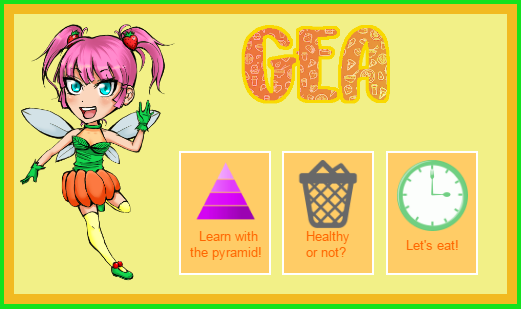
\includegraphics[width=10cm, height=6cm]{immagini/Game.png}
\caption{Home page}\label{fig:home}
\end{figure}
\begin{figure}[H]
\centering
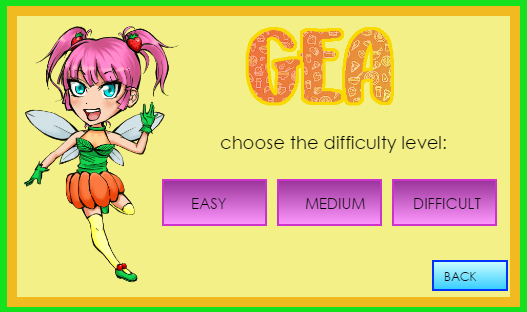
\includegraphics[width=10cm, height=6cm]{immagini/Level.png}
\caption{Level page}\label{fig:level}
\end{figure}
In figure \ref{fig:homeflow} is shown the flow diagram of the application. As described above the app starts, then there are game's choice and relative selection of difficulty, finally the mini-game is launched. At the end of the session it comes back to the home page.
\begin{figure}[H]
\centering
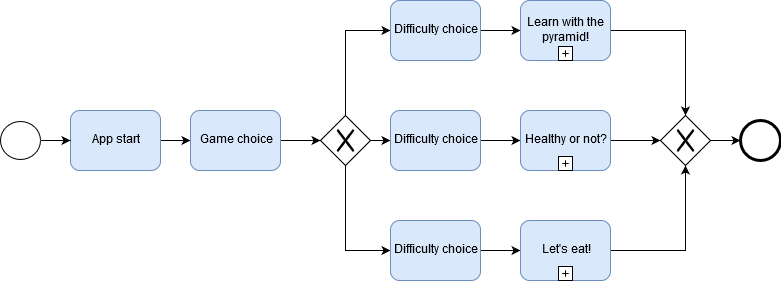
\includegraphics[width=15cm, height=5cm]{immagini/flow1.png}
\caption{Home page flow diagram}\label{fig:homeflow}
\end{figure}
When the game starts, the patient is immersed in the virtual space, which is the same for all the games and reproduces the real setting of the therapy: there is a room with a table, a fridge, a window,a door, a sofa and a kitchen, in order to keep the space as simple as possible but also inherent with nutrition. In front of the user, a short explanation for each game and a play button appear. The explanation is represented by graphical clues, to be understandable also by users who cannot read. Moreover, a fantasy character serving as mascot of the game was created, with the goal of making the application more fun and serving as visual feedback after each user's action. At the end of each session with each game the number of correct and wrong answers is shown to the user, with the total scored points.\\
In figure \ref{fig:gameflow} is shown the flow diagram of each mini-game, they are all structured with the start and appearing of the choices. After that the user as to select what he/she thinks is correct and a feedback confirm or not with a respective increment or not of the points. At the end of three or five session (depending on the game) the total score is displayed and after some seconds the app come back to the home page.
\begin{figure}[H]
\centering
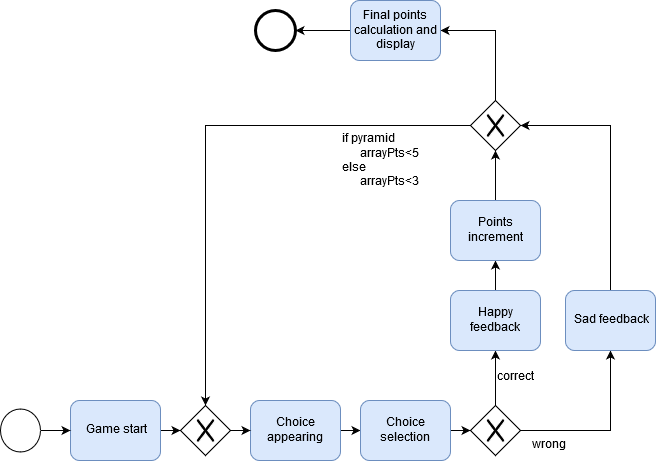
\includegraphics[width=15cm, height=8cm]{immagini/flow2.png}
\caption{Games flow diagram}\label{fig:gameflow}
\end{figure}
\subsection{"Learn with the pyramid!" page}
This game aims to teach how to complete the food pyramid, by selecting which food goes in each level. In the virtual environment appears a pyramid divided into five levels, with a pointer indicating which level the user is currently completing and the table with three options \ref{fig:pyramid}. The red circle in the image is the pointer representing the current user's focus point. The user has to focus on the correct choice for a certain time interval to give the answer, avoiding possible unwanted answers while the user is looking around in the environment. After an answer is given, a feedback is provided: the game mascot appears with a sad expression if the answer is wrong and the active level of the pyramid becomes red, if the answer is correct a happy mascot is shown and the level becomes green.
\begin{figure}[H]
\centering
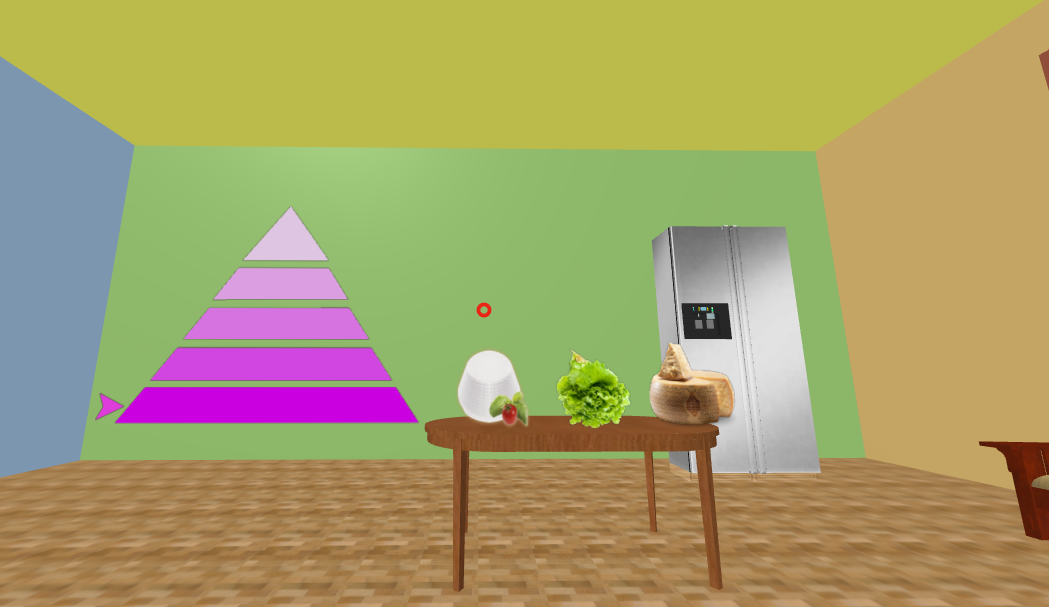
\includegraphics[width=10cm, height=6cm]{immagini/Pyramid.png}
\caption{"Learn with the pyramid!" page}\label{fig:pyramid}
\end{figure}
\subsection{"Healthy or not?" page}
This game is proposed to train patients in recognizing if a dish is healthy or not. When the game starts, two dishes appear on the table of the virtual room, with a bin and the visual explanation of how the game works \ref{fig:healthy}: the user must select the "junk food" with the eyes and move it, by keeping the gaze focused on it, until it is thrown in the bin. There are three repetitions of this game, with different choices, and after each answer a feedback is shown, like the one described before.
\begin{figure}[H]
\centering
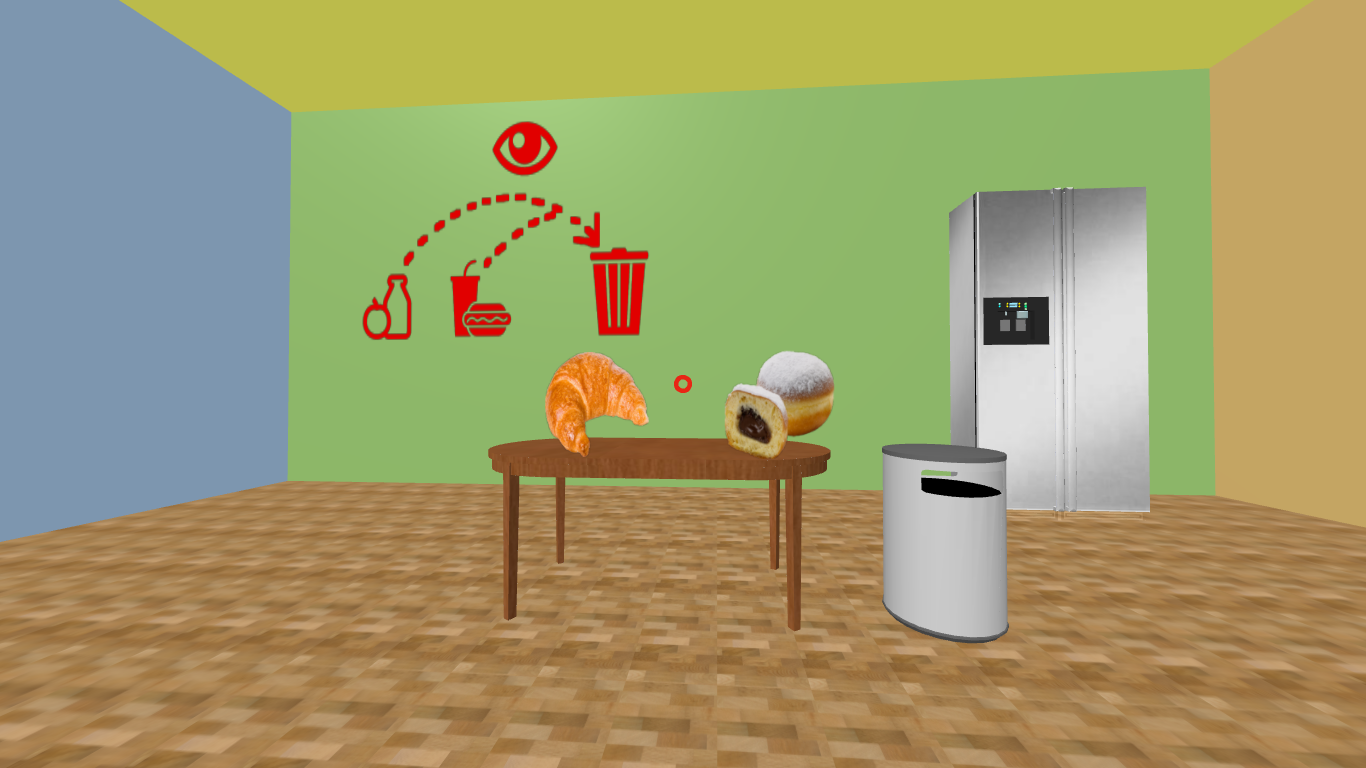
\includegraphics[width=10cm, height=6cm]{immagini/Healthy.png}
\caption{"Healthy or not?" page}\label{fig:healthy}
\end{figure}
\subsection{"Let's eat!" page}
This game aims to teach how to associate meals of the day to specific dishes. It was created in particular
for those patients who have difficulties in understanding when they can eat something or they cannot. In this case, the virtual environment presents four images representing the four main meals (breakfast, lunch, afternoon snack and dinner) and a dish \ref{fig:eat}: the goal is to select the correct meal/s in which the dish can be eaten. Like in the second game, there are three repetitions and after each answer a feedback is given.
\begin{figure}[H]
\centering
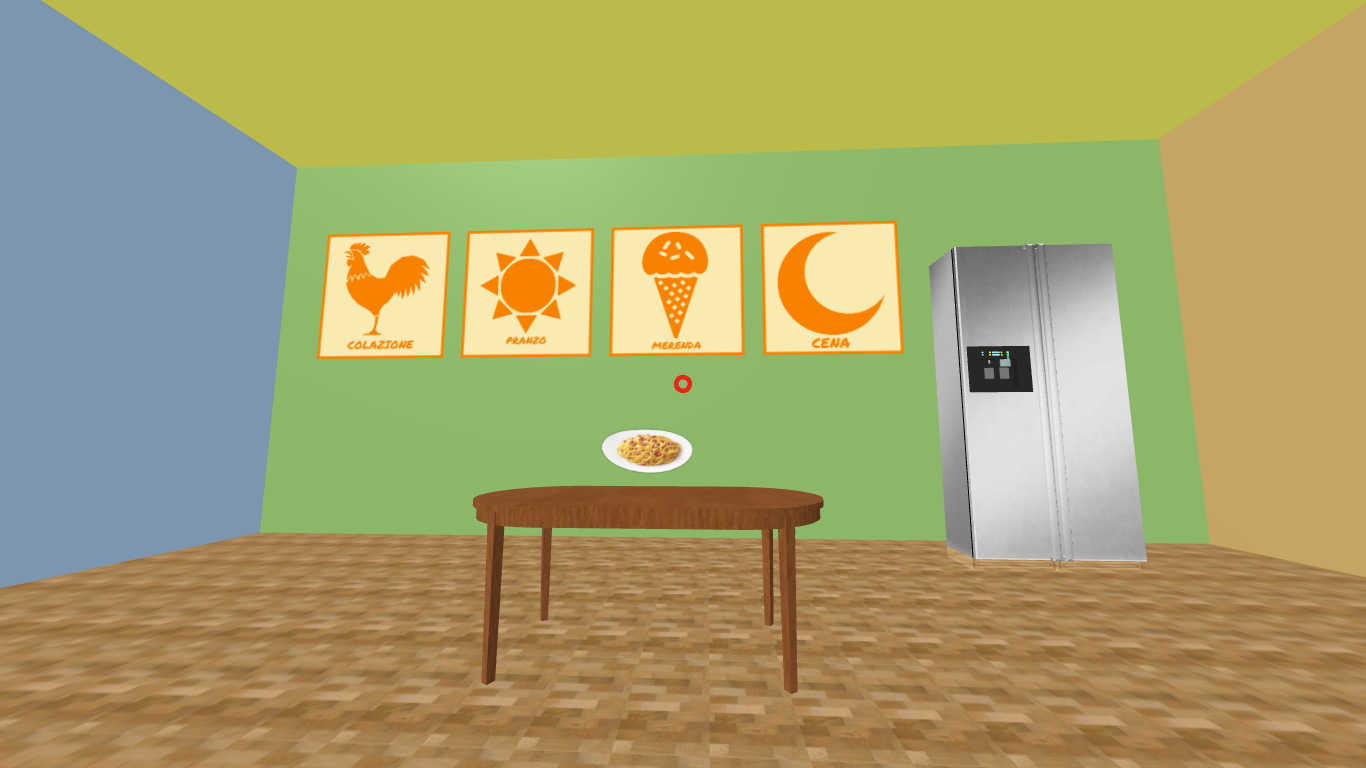
\includegraphics[width=10cm, height=6cm]{immagini/Eat.png}
\caption{"Let's eat!" page}\label{fig:eat}
\end{figure}

\section{Implementation Overview}